\documentclass[a4paper,11pt]{jsarticle}

%まず使用するパッケージ
\usepackage{amsmath, amsfonts, amssymb, mathtools, mathrsfs, latexsym}
\usepackage{nccmath, empheq}

%\usepackage[draft]{graphicx}
\usepackage[dvipdfmx]{graphicx}
\usepackage[dvipdfmx]{color}
\usepackage{here, wrapfig, subcaption}
\usepackage{enumerate, comment, fancyhdr}
\usepackage{otf}
%mathtoolsを用いたコマンド定義
\DeclarePairedDelimiter{\abs}{\lvert}{\rvert}

\usepackage{seiritz}

\pagestyle{fancy}
  \lhead{2023/12/23}
  \rhead{第3問}
  \cfoot{\thepage}

%%%%%%%%%% メイン %%s%%%%%%%%
\begin{document}
\qSentence{第3問}
%!TEX root = *.tex
%%%%%%%%%%%%%%%%%%
% カウンタのリセット
\setcounter{figure}{0}
% 問題文
\noindent\textsf{\bfseries A}\ 
図1のように屈折率$n_1$の媒質\ajRoman{1}と屈折率$n_2$の媒質\ajRoman{2}が水平な境界面で接している.
いま,点A,Bがそれぞれ媒質\ajRoman{1},\ajRoman{2}中にある場合を考える.
点Aは点Bの真上にあり,点A,Bはそれぞれ境界面から距離$d_1$,$d_2$ だけ離れた位置にある.
媒質\ajRoman{2}中の点Bを始点として長さ$l$の棒を水平に置き, 
この棒を点Aから見ることを考える.
棒の他端の位置を点Cとし,点Cを出て点Aに到達する光
が媒質\ajRoman{2}から媒質\ajRoman{1}に入射する際の入射角を$i$,屈折角を$r$とする.棒の長さ$l$は距離$d_1,d_2$に対して十分小さく,
したがって$i,r$も十分小さい.
屈折率は$n_2>n_1$である.
なお,角度はラジアンを単位として表すものとし,
必要であれば,$\theta\,(\theta>0)$が十分小さいときに成り立つ近似式$\sin\theta=\tan\theta=\theta$を用いてよい.



\begin{enumerate}[(1)]
  \setlength{\leftskip}{-1zw}
  \setlength{\itemindent}{1zw}\setlength{\labelsep}{0.5zw}
  \setlength{\labelwidth}{1zw}\setlength{\leftmargin}{1zw}
  \setlength{\itemsep}{0.5\baselineskip}
  \item 点Aから見ると棒の他端は図1の点$\C^\prime$の方向に見える.
  $\B\C^\prime$の長さを点Aから見た棒の見かけの長さとする
  (以下でも同様とする).
  この見かけの長さを$d_1,\,d_2,\,n_1,\,n_2,\,l$を用いて表しなさい.
\end{enumerate}


\begin{enumerate}[(1)]
  \setlength{\leftskip}{-1zw}
  \setlength{\itemindent}{1zw}\setlength{\labelsep}{0.5zw}
  \setlength{\labelwidth}{1zw}\setlength{\leftmargin}{1zw}
  \setlength{\itemsep}{0.5\baselineskip}
  \addtocounter{enumi}{1}
  \item 次に,図2のように長さ$l$の棒を媒質\ajRoman{1}の中に点Aを始点として水平に置いた.点Bから見た棒の見かけの長さを$d_1,\,d_2,\,n_1,\,n_2,\,l$を用いて表しなさい.
\end{enumerate}


\begin{enumerate}[(1)]
  \setlength{\leftskip}{-1zw}
  \setlength{\itemindent}{1zw}\setlength{\labelsep}{0.5zw}
  \setlength{\labelwidth}{1zw}\setlength{\leftmargin}{1zw}
  \setlength{\itemsep}{0.5\baselineskip}
  \addtocounter{enumi}{2}
  \item 棒の長さ$l$をどれだけ長くしても,点Bから見た棒の見かけの長さはある長さ$l_1$より長くなることはなかった.
$l_1$を$d_1,\,d_2,\,n_1,\,n_2,$を用いて表しなさい.ただしこの場合は入射角や屈折角が十分小さいとは限らないことに注意しなさい.
\end{enumerate}



\begin{enumerate}[(1)]
  \setlength{\leftskip}{-1zw}
  \setlength{\itemindent}{1zw}\setlength{\labelsep}{0.5zw}
  \setlength{\labelwidth}{1zw}\setlength{\leftmargin}{1zw}
  \setlength{\itemsep}{0.5\baselineskip}
  \addtocounter{enumi}{3}
  \item 媒質\ajRoman{2}の下に水平な境界面で接している屈折率$n_3\,(n_3>n_2)$の媒質\ajRoman{3}がある場合を考える.
媒質\ajRoman{2}と媒質\ajRoman{3}の境界から距離$d_3$だけ離れた媒質\ajRoman{3}の中に長さ$l$の棒を境界面に水平に置いた.
棒の始点は点Aの真下にある.点Aから見た棒の見かけの長さ$d_1,\,d_2,\,d_3,\,n_1,\,n_2,\,n_3,\,l$を用いて表しなさい.ただし,$l$は$d_3$に比べて十分小さい.
\end{enumerate}



\begin{figure}[H]
  \centering
  \begin{minipage}{.3\columnwidth}
    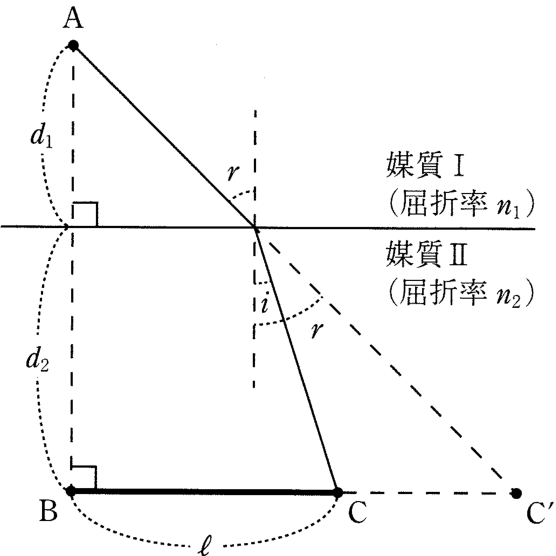
\includegraphics[width=\columnwidth]{../graphs/chiba_23_6-1.png}
    \caption{}
  \end{minipage}
  \hspace{.1\columnwidth}
  \begin{minipage}{.3\columnwidth}
    \centering
    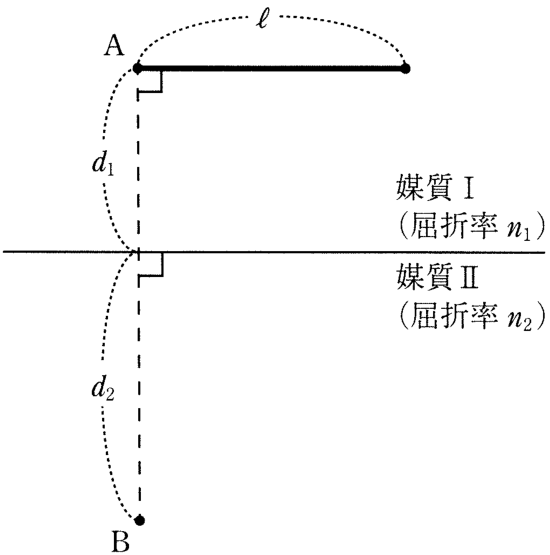
\includegraphics[width=\columnwidth]{../graphs/chiba_23_6-2.png}
    \caption{} 
  \end{minipage}
\end{figure}

\noindent\textsf{\bfseries B}
\ 
反射と屈折の法則は,
「光がある点から別の点まで進むとき,所要時間が最小になるような経路をとる」
というフェルマーの原理から導くことができる.

\begin{enumerate}[(1)]
  \setlength{\leftskip}{-1zw}
  \setlength{\itemindent}{1zw}\setlength{\labelsep}{0.5zw}
  \setlength{\labelwidth}{1zw}\setlength{\leftmargin}{1zw}
  \setlength{\itemsep}{0.5\baselineskip}
  \addtocounter{enumi}{4}
  \item 図3のように\x 軸上に平面鏡を置き,平面鏡に垂直で図の上向きに\y 軸をとる.
  \xy 平面上にある2点A,Bを考え,それぞれの位置を\mbox{$(a_x,\,a_y)$},\mbox{$(b_x,\,b_y)$}とする.
  点Aから出た光が平面鏡で反射して点Bに到達するとき,光は\x 軸上のどこで反射されるかを考える.
  光の道筋は\xy 平面にあるものとし,反射する点の\x 座標を$a_x,\,a_y,\,b_x,\,b_y$を用いて表しなさい.
  ただし,$a_x,\,a_y,\,b_x,\,b_y$はすべて正である.
  \item 次の文章の空欄\BrankNo{(ア)}$\sim$\BrankNo{(カ)}に適切な式を入れなさい.ただし,解答に用いる物理量を表す記号は,以下の文章中に与えられているものとする.\par 
  \vspace{.5\baselineskip}\quad 
  図4のように屈折率$n_1$の媒質\ajRoman{1}と屈折率$n_2$の媒質\ajRoman{2}が水平な境界面で接している.
  媒質\ajRoman{1}中の点Aを出た光が媒質\ajRoman{2}中の点Bに到達する場合を考える.
  光は点Bに到達するまでの時間が最小になるように媒質の境界面上の点を通過する.
  この通過点を点Oとする.以下では屈折率は$n_2>n_1$とする.\par \quad 
  いま,点Oを原点とし,2点A,Bが\xy 面内に含まれる境界面内に\x 軸,
  これと垂直に\y 軸をとる.
  A,Bの座標をそれぞれ$(-a_x,\,a_y)$,$(b_x,\,-b_y)$とする.
  ただし,$a_x,\,a_y,\,b_x,\,b_y$はすべて正である.\par\quad 
  真空中の光の速さを$c$とすると,媒質\ajRoman{1}中の光の速さは\BrankNo{(ア)}であるので,光が経路AOを進むのに要する時間は\BrankNo{(イ)}となる.
  同様にして経路OBを進むのに要する時間も求めることができ,光が経路AOBを進むのに要する時間は\BrankNo{(ウ)}となる.\par\quad 
  次に,光は点Oからわずかにずれた点$\O^\prime\,(\Delta x,\,0)$を通ると仮定する.
  すると,経路$\A\O^\prime$および経路$\O^\prime\B$の距離はそれぞれ\BrankNo{(エ)},\BrankNo{(オ)}となる.
  光が経路AOBに対して経路$\A\O^\prime\B$を進む場合の所要時間の増分を$\Delta t$とする.
  $\Delta x$が十分に小さいため,$(\Delta x)^2$が無視できることを考慮した上で$h$の絶対値が十分に小さいときに成り立つ近似式$\sqrt{1+h}\fallingdotseq 1+\dfrac{h}{2}$を用いることにより,$\dfrac{\Delta t}{\Delta x}$は\BrankNo{(カ)}と求まる.
  ここで,$\dfrac{\Delta t}{\Delta x}=0$となるという条件を課すと,屈折の法則を導くことができる.
\end{enumerate}

\begin{figure}[H]
  \centering
  \begin{minipage}{.3\columnwidth}
    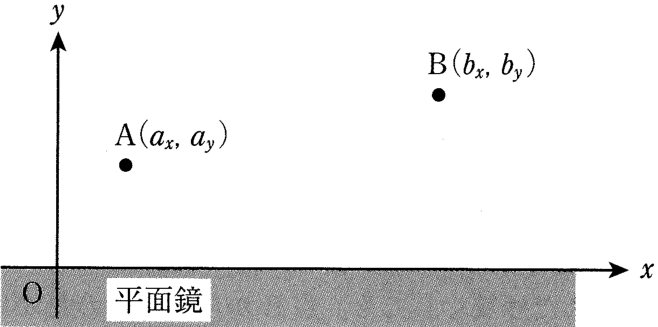
\includegraphics[width=\columnwidth]{../graphs/chiba_23_6-3.png}
    \caption{}
  \end{minipage}
  \hspace{.1\columnwidth}
  \begin{minipage}{.3\columnwidth}
    \centering
    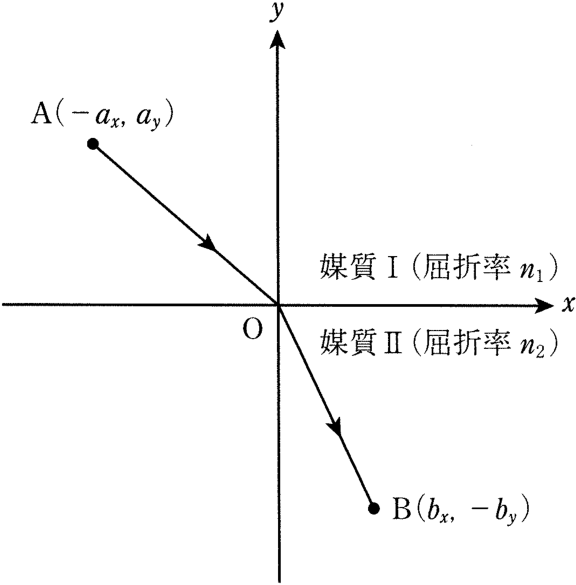
\includegraphics[width=\columnwidth]{../graphs/chiba_23_6-4.png}
    \caption{} 
  \end{minipage}
\end{figure}

% メモ
\begin{comment}

\end{comment}


%%%%%%%%%%%%%%%%%%

\hruleline
%\input{../prac_exam/open_19_8/Q2_sol.tex}
\end{document}